\documentclass[a4paper,11pt]{article}
\pdfoutput=1 % if your are submitting a pdflatex (i.e. if you have
             % images in pdf, png or jpg format)

\usepackage{jinstpub} % for details on the use of the package, please
                     % see the JINST-author-manual

\usepackage{amsmath}

\title{\boldmath  Cerium-doped Fused-silica Fibers
as Wavelength Shifters}


%% %simple case: 2 authors, same institution
%% \author{A. Uthor}
%% \author{and A. Nother Author}
%% \affiliation{Institution,\\Address, Country}

% more complex case: 4 authors, 3 institutions, 2 footnotes
\author[a,1]{N.~Akchurin,\note{Corresponding author.}}
\author[a]{J.~Damgov,}
\author[a]{F.~De Guio,}
\author[c]{G.~Dissertori,}
\author[b]{E.~Kendir,}
\author[a]{S.~Kunori,}
\author[a]{T.~Mengke,}
\author[c]{F.~Nessi-Tedaldi,}
\author[d]{N. Pastrone,}
\author[c]{S.~Pigazzini,}
\author[b]{\c{S}.~Yaltkaya}

\affiliation[a]{Texas Tech University, Department of Physics and Astronomy,  Lubbock, TX, 79409, USA}
\affiliation[b]{Akdeniz University, Department of Physics, Antalya, 07070, Turkey}
\affiliation[c]{ETH, Z\"urich, Switzerland}
\affiliation[d]{INFN-Torino, Italy}
% e-mail addresses: only for the forresponding author
\emailAdd{nural.akchurin@ttu.edu}

\abstract{
We evaluated the performance of a Ce-doped fused-silica fiber as wavelength shifter coupled to a CeF$_3$ crystal using electron beams at CERN.   The pulse shape and collection efficiency were measured using irradiated (10 MRad) and un-irradiated fibers.  In addition, we evaluated the light yield of various Ce-doped fibers and explored the possibility of using these types of ``hybrid'' fibers for future precision timing applications in high-luminosity environment.
}

\keywords{Cerium, optical fibers, fused silica}

\begin{document}
\maketitle
\flushbottom


\section{Introduction}
\label{sec:intro}
We described our results from five prototype Ce-doped fibers in two previous publications:  in the first paper~\cite{JINSTPaper}, we concentrated on the scintillation pulse shape, light yield, attenuation length, and the differences between the scintillation light and Cherenkov radiation.  In the second paper~\cite{JINSTPaper2}, we focused on fiber morphology, chemical composition, photo- and radio-luminescence, radiation-damage induced attenuation measurements and its modeling based on rate equations, and the evaluation of changes in effective numerical aperture under gamma irradiation.   In all our studies, we included clear fused-silica fiber containing no dopants  as benchmark.   In this paper, we present our results on the use of Ce-doped fibers, both irradiated and un-irradiated, as wavelength shifters when coupled to a single Cerium Fluoride (CeF$_3$) crystal using high energy electron beams at CERN.  We also evaluated the performance of these fibers for use in precision timing detectors and compared them to common plastic scintillators and to a Cherenkov radiator (clear fused-silica fiber).  With these measurements, we were able to confirm and improve our previous light yield estimates.  All fibers reported here are produced by Polymicro Technologies\footnote{Polymicro Technologies is a subsidiary of Molex located in Phoenix, AZ, USA.}.

\section{Experimental Setup}
\label{sec:experimentalsetup}
The test has been performed in the H4 beam line of the CERN SPS North Area. There, the electron momentum spread that can be achieved is given by the momentum defining collimators: when they are closed to $\pm 3$ mm, the momentum spread of the beam is calculated to be less than $0.2\%$\cite{r-GRA}. 
The high-energy electrons there are tracked by a spectrometer for obtaining a precise impact point: a wire-chamber (placed at 12 m from the tested setup), two scintillating-fibre hodoscopes (placed at 6 and 3 m distance). The wire chamber is made of two planes of 55 cathode wires and 28 anode wires, organized in a grid with an active area of $80\times 80$ mm$^2$. Each plane provides, respectively, a measurement of the electron position in the x and y directions with a nominal resolution better than 200 $\mu$m~\cite{r-SPA}.
Each of the two scintillating-fibre hodoscopes is built of two layers of 64 plastic fibres with diameter 0.5 mm, oriented in the x and y directions, respectively. The signals from the fibres are clustered grouping together adjacent fibres, up to a maximum of 4 fibres per cluster. The cluster position is defined as the average position of its fibres and it is used to estimate the trajectory of the particle before the impact.
Four plastic scintillators of varying size, the smallest of which has a transverse dimension of $1 \times 1$ cm$^2$, are placed in the beamline for triggering purposes.

Test beam data have been acquired with a custom developed DAQ system~\cite{r-MAR}. The core system has been built around the ZeroMQ library, which provide a low latency communication over ordinary networks allowing to operate several instances of the DAQ on different machines. A typical  configuration used during the tests described  herein included a master application interfaced to the SPS communication system and a slave instance, running on a PC close to the setup, which read out the data from the detectors. Although the DAQ system is built with a general API that can be interfaced to different hardware throughout the beam test we extensively used the CAEN V1742 VME board. The V1742 includes 4 DRS4 chips that allow one to sample the detector signal at frequency up to 5 GHz. The choice of this flexible configuration enabled us to optimize the signal reconstruction offline.

The detailed information on the fibers used in the tests can be found in~\cite{JINSTPaper}.  Table~\ref{tab:fiberlist} summarizes the physical dimensions while Figure~\ref{fig:FiberCrossSections} shows fiber cross-sectional images.  Some performance characteristics of Phase-I and -II fibers that were measured with the high energy beams at Fermilab were reported in our first paper \cite{JINSTPaper}.  For example, the Phase-I optical attenuation length measured about $5.8\pm0.7$ m using 16 GeV  electrons.  The speed of light propagation was $19.50\pm0.38$ cm/ns and was found to be consistent with the previously reported values \cite{Goro,Akch97}.  When the tail of the pulse was modeled by a sum of two exponential functions, two decay constants were obtained, $\tau_1= 20.8\pm5.4$, and $\tau_2= 93.0\pm12.6$ ns.  The contributions of these components to the total light emission (radioluminescence) turned out to be $23.9\pm5.3$\% and $76.1\pm5.3$\%, respectively.  In our second paper \cite{JINSTPaper}, we focused on the fiber chemical compositions and their impact on their radiation-hardness properties.  We also showed that the radiation induced attenuation and recovery can be successfully modeled by a set of self-consistent kinematic rate equations.

\begin{table}[htp]
\caption{\small List of investigated fibres, with their characteristics. All fibers were cladded with fluorinated acrylate and UV-cured acrylate buffer.}
\vspace{-2 mm}
\begin{center}
{\small
\begin{tabular}{|l|c|c|c|c|c|c|c|c|} \hline
Fiber              &  Core OD            & Glass OD        & Clad OD          & Buffer  OD        \\
Name               &[${\rm \mu m}$]      & [${\rm \mu m}$] & [${\rm \mu m}$]  & [${\rm \mu m}$]   \\
\hline
Phase-I            & 60$\pm$7            &	200$\pm$6      & 230$^{+5}_{-10}$ &	350$\pm$15        \\
Phase-II           & 150$\pm$20		     &	400$\pm$10     & 430$\pm$10	      &	550$\pm$30        \\
%Phase-III          & 370$\pm$8			 &	 -             & 400 $\pm$8 	  &	550$\pm$15        \\
Phase-IV           & 200$\pm$8(clear)   &	600$\pm$6	   & 630$\pm$10       &	800$\pm$30        \\
                          & 230$\pm$8(doped) &	   &     &	         \\
Clear fused-silica & 600$\pm$10          &-				   & 630$^{+5}_{-10}$ &	800$\pm$30	      \\
%T14                & 150$\pm$5	         &	400$\pm$5	   & 450$\pm$5        & 500$\pm$15	      \\
                    &                     &                &                  & \\
\hline
\end{tabular}
}
\end{center}
\label{tab:fiberlist}
\end{table}


\begin{figure}[ht]
\begin{center}\vspace{-1pc}
      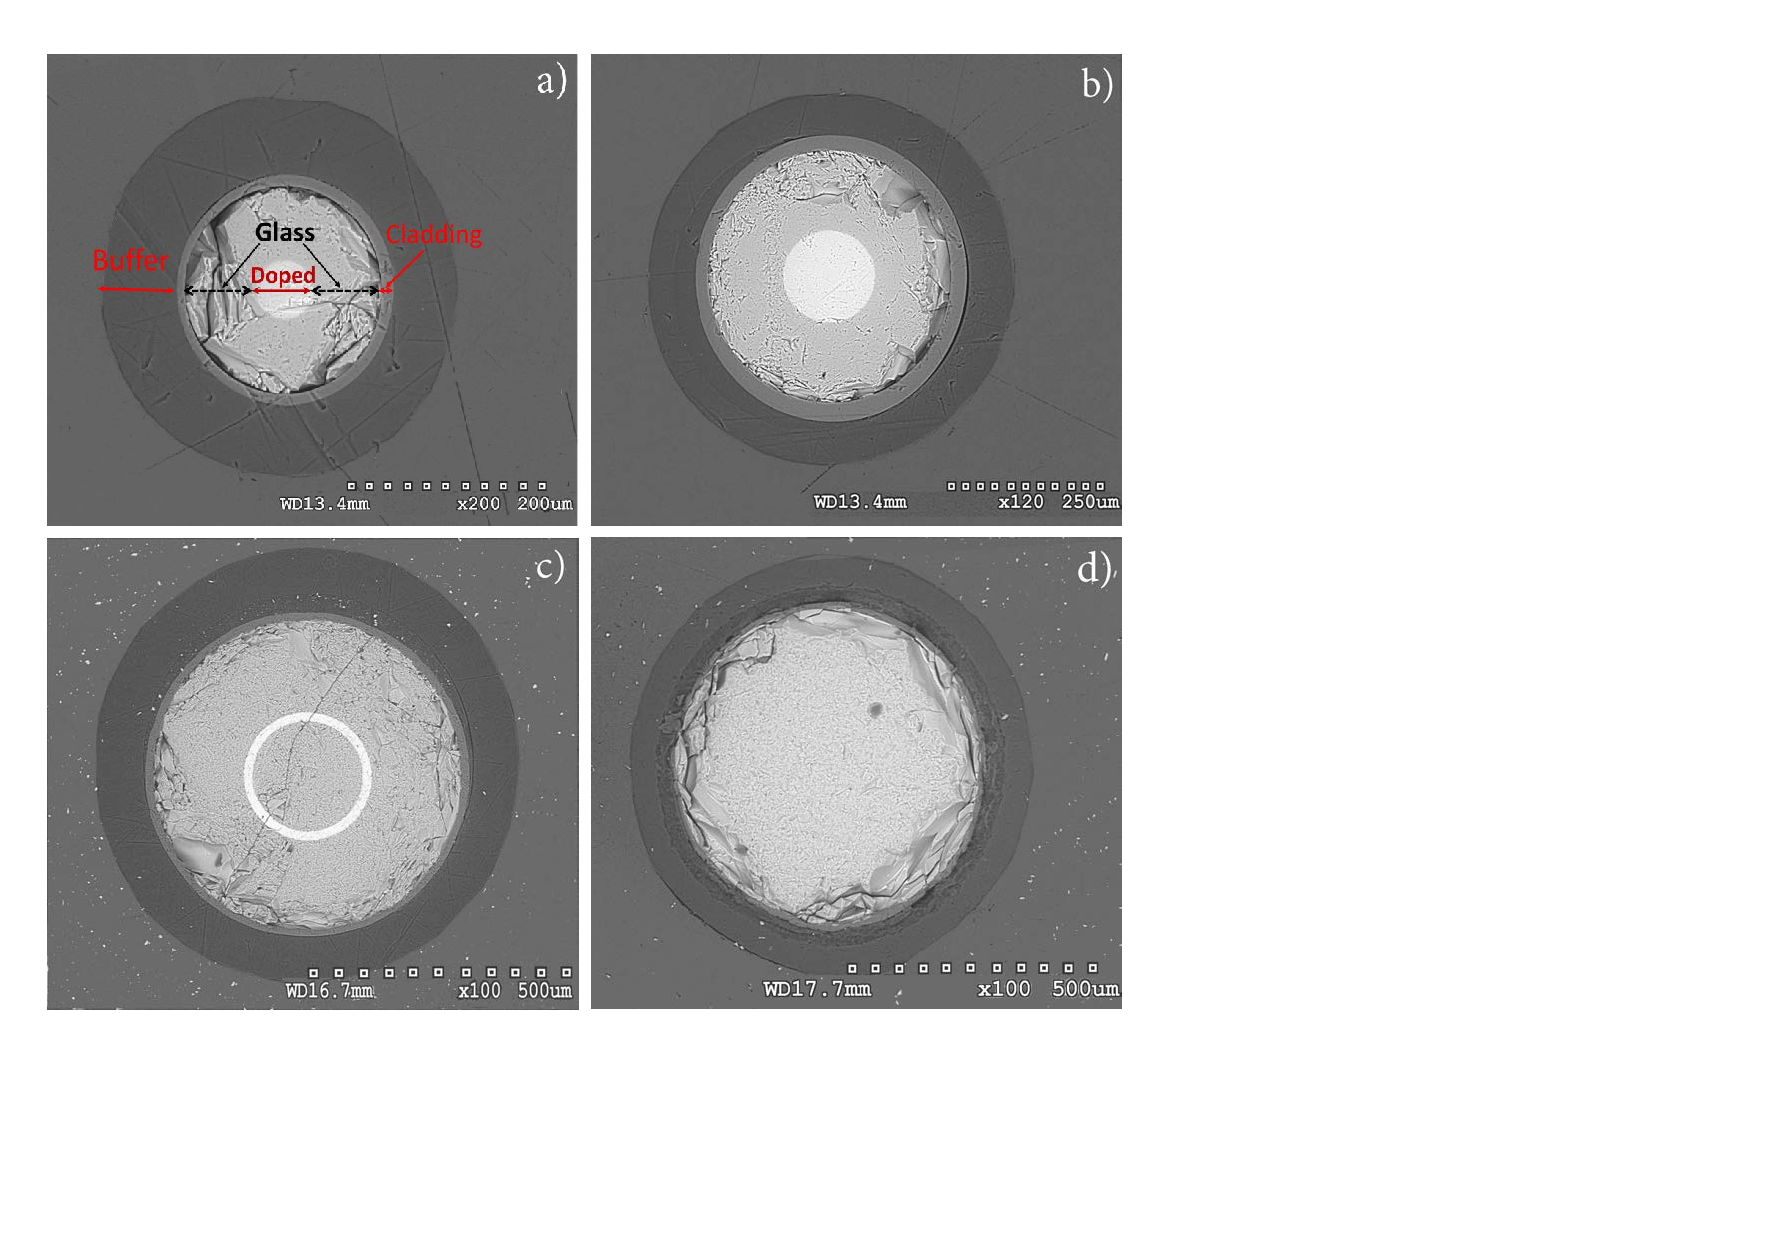
\includegraphics[width=10 cm]{Figures/allfiberimage2.pdf}
\caption{\small The cross-section of fibers
{\it a)} Phase-I,
{\it b)} -II,
{\it c)} -IV, and
{\it d)} clear fused-silica are shown.  The terminology used throughout the paper for different parts of the fiber is indicated on {\it a)}.}
    \label{fig:FiberCrossSections}
\end{center}
\end{figure}

\section{Scintillation Light Yield Measurements}
\label{sec:lightyield}
The light yield is an important characteristics of the fibers. The method we adopted for this measurement is the same used in the first paper~\cite{JINSTPaper}. 

For this measurement the fibers were bundled, placed in aluminum tubes and exposed to an electron beam with energy of 16 GeV at 90 degree (Fig.~\ref{fig:bundles}). In front of the bundles a brass block with 4~cm thickness was placed, corresponding to about 2.7 $X_0$. The light was collected by photomultiplier tubes (Hamamatsu R6427). The photomultiplier (PMT) signals were read out by a fast digitizer (CAEN V1742) at 2.5 GHz and a common trigger was generated by a fast multichannel photomultiplier (MCP). Each bundle contained only one type of fibers: 6 Phase-IV unirradiated, 6 Phase-IV irradiated, 85 Phase-II or 61 clear fibers. The absolute light yield is measured in photo-electrons per event. The calibration is set with single photo-electron measurement for each PMT individually. We use the timing characteristics of the Cherenkov (Q) and scintillation (S) signals to integrate them individually. We measured Q = 0.092 p.e. and S = 0.147 p.e. for the unirradiated Phase-IV fiber bundle. For irradiated Phase-IV fibers we obtained Q = 0.058 p.e. and S = 0.62 p.e. 
These infers that after the irradiation the Cherenkov light yield is reduced. However, the measured scintilation light yield increased by a factor of four. For the Phase-II fiber bundle we measure Q = 0.44 p.e. and S = 2.25 p.e. on average per event.

\begin{figure}[ht]
\begin{center}\vspace{-1pc}
      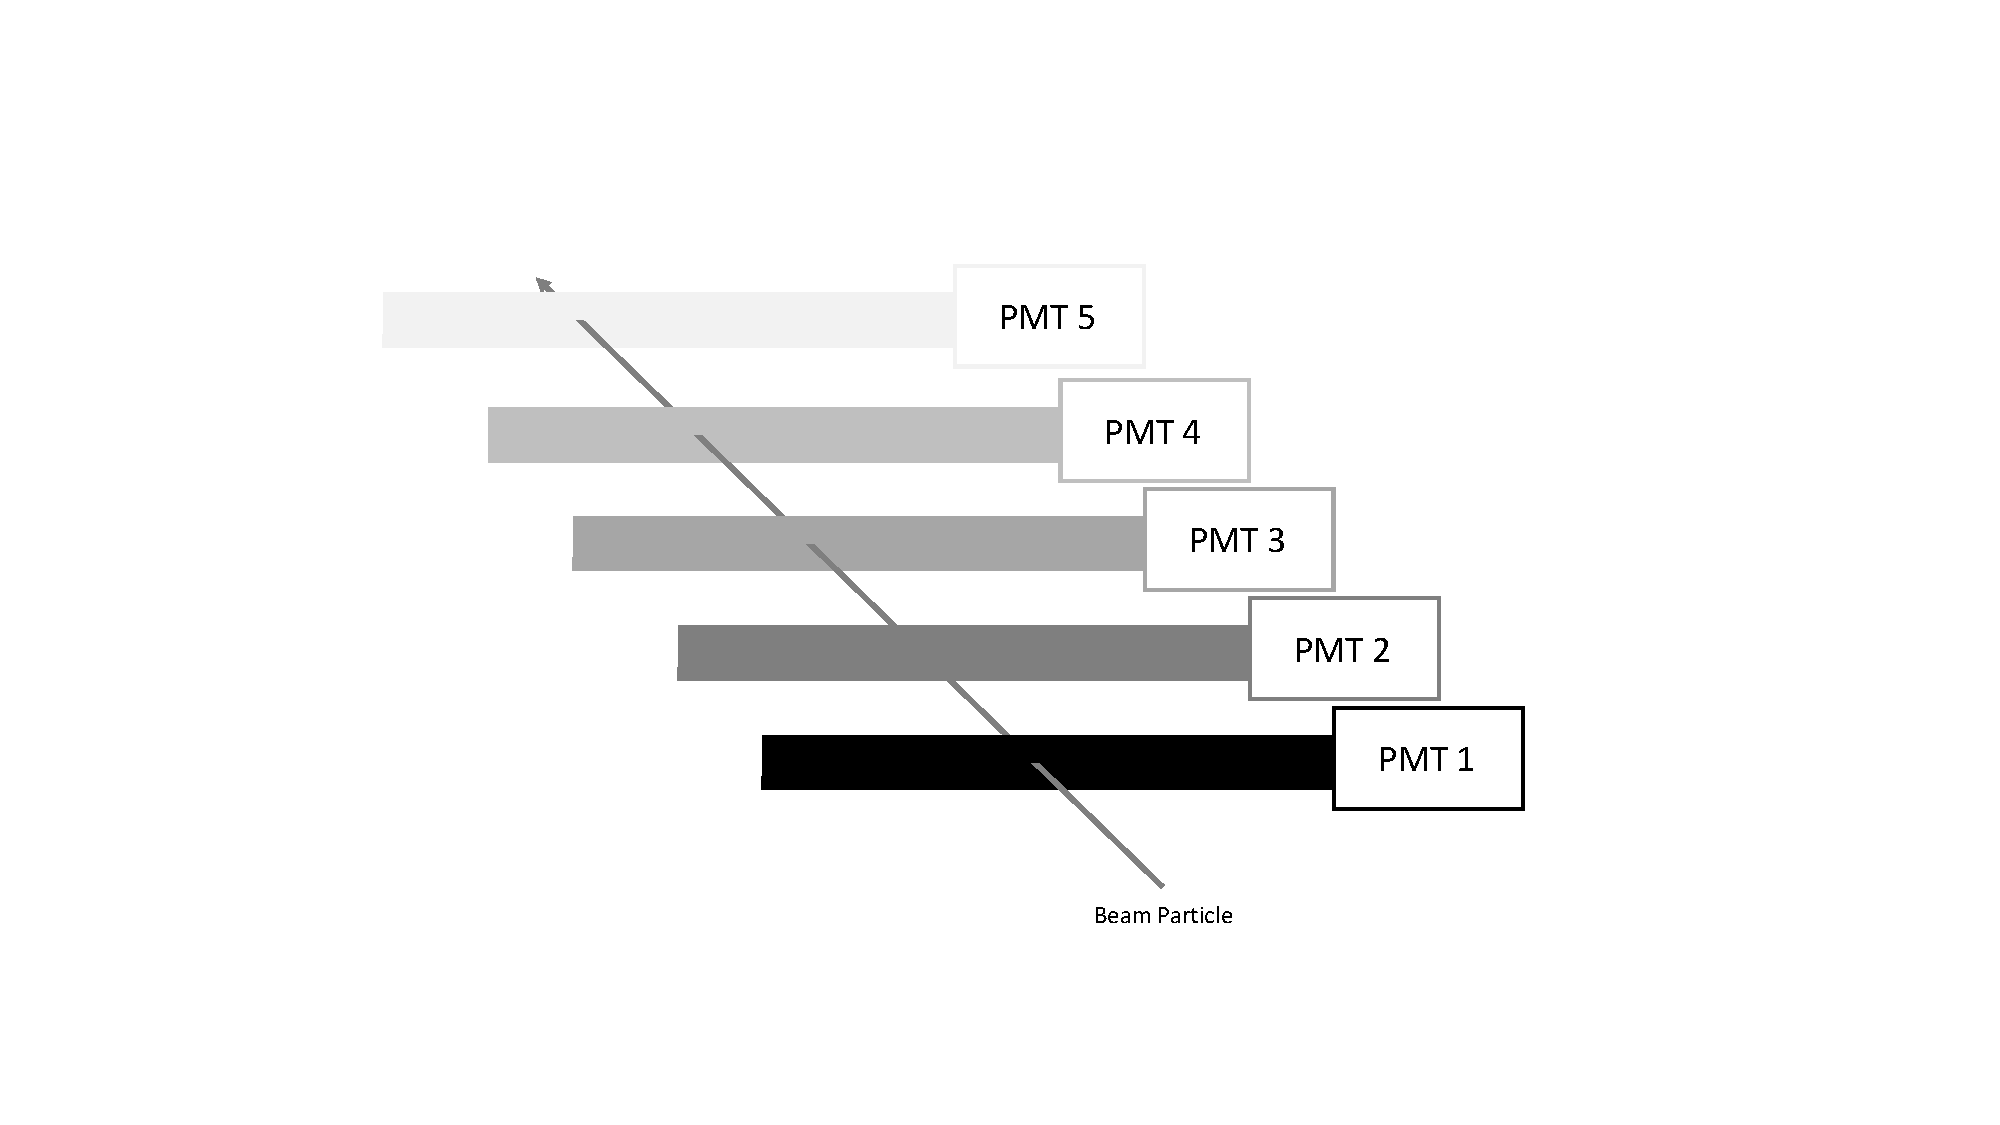
\includegraphics[width=10cm]{Figures/FiberBundles.pdf}
       %%\vspace{-1pc}
\caption{\small Bundles.....}
    \label{fig:bundles}
\end{center}
\end{figure}

We used the GEANT4 simulation to translate these measurements into a characteristic scintillation light yield for the Ce-doped silica. We compare the measured S/Q ratio with the prediction from the simulation for a  known scintillation light yield. This approach (using the S/Q ratio) results in canceling out many of the systematic uncertainties related to the measurement of the individual components of the signal. The scintillation mechanism in simulations is implemented as 500 photons produced isotropically per MeV of energy deposited via ionization losses from charged particles in the Ce-doped silica. The wavelength of these photons is  matched to the measured spectrum in data (Fig.~\ref{??}). In the GEANT4 simulation we implemented the full geometry if the setup, a detailed description of light propagation and the characteristics of the photodetectors. 
As a result the measured characteristic scintillation light yield for the Ce-doped silica is $820\pm 360$ photons/MeV for unirradiated Phase-IV fibers. 

We also measured the timing characteristics of the scintillation component of the signals for Phase-IV fiber. We found that the single exponent describes best the tails (Fig.~\ref{fig:phase4scintTime}). The time constants are $119.3 \pm 20.7$ ns and $102.3 \pm 10.3$ ns for unirradiated and irradiated fibers respectively.

\begin{figure}[ht]
\begin{center}
      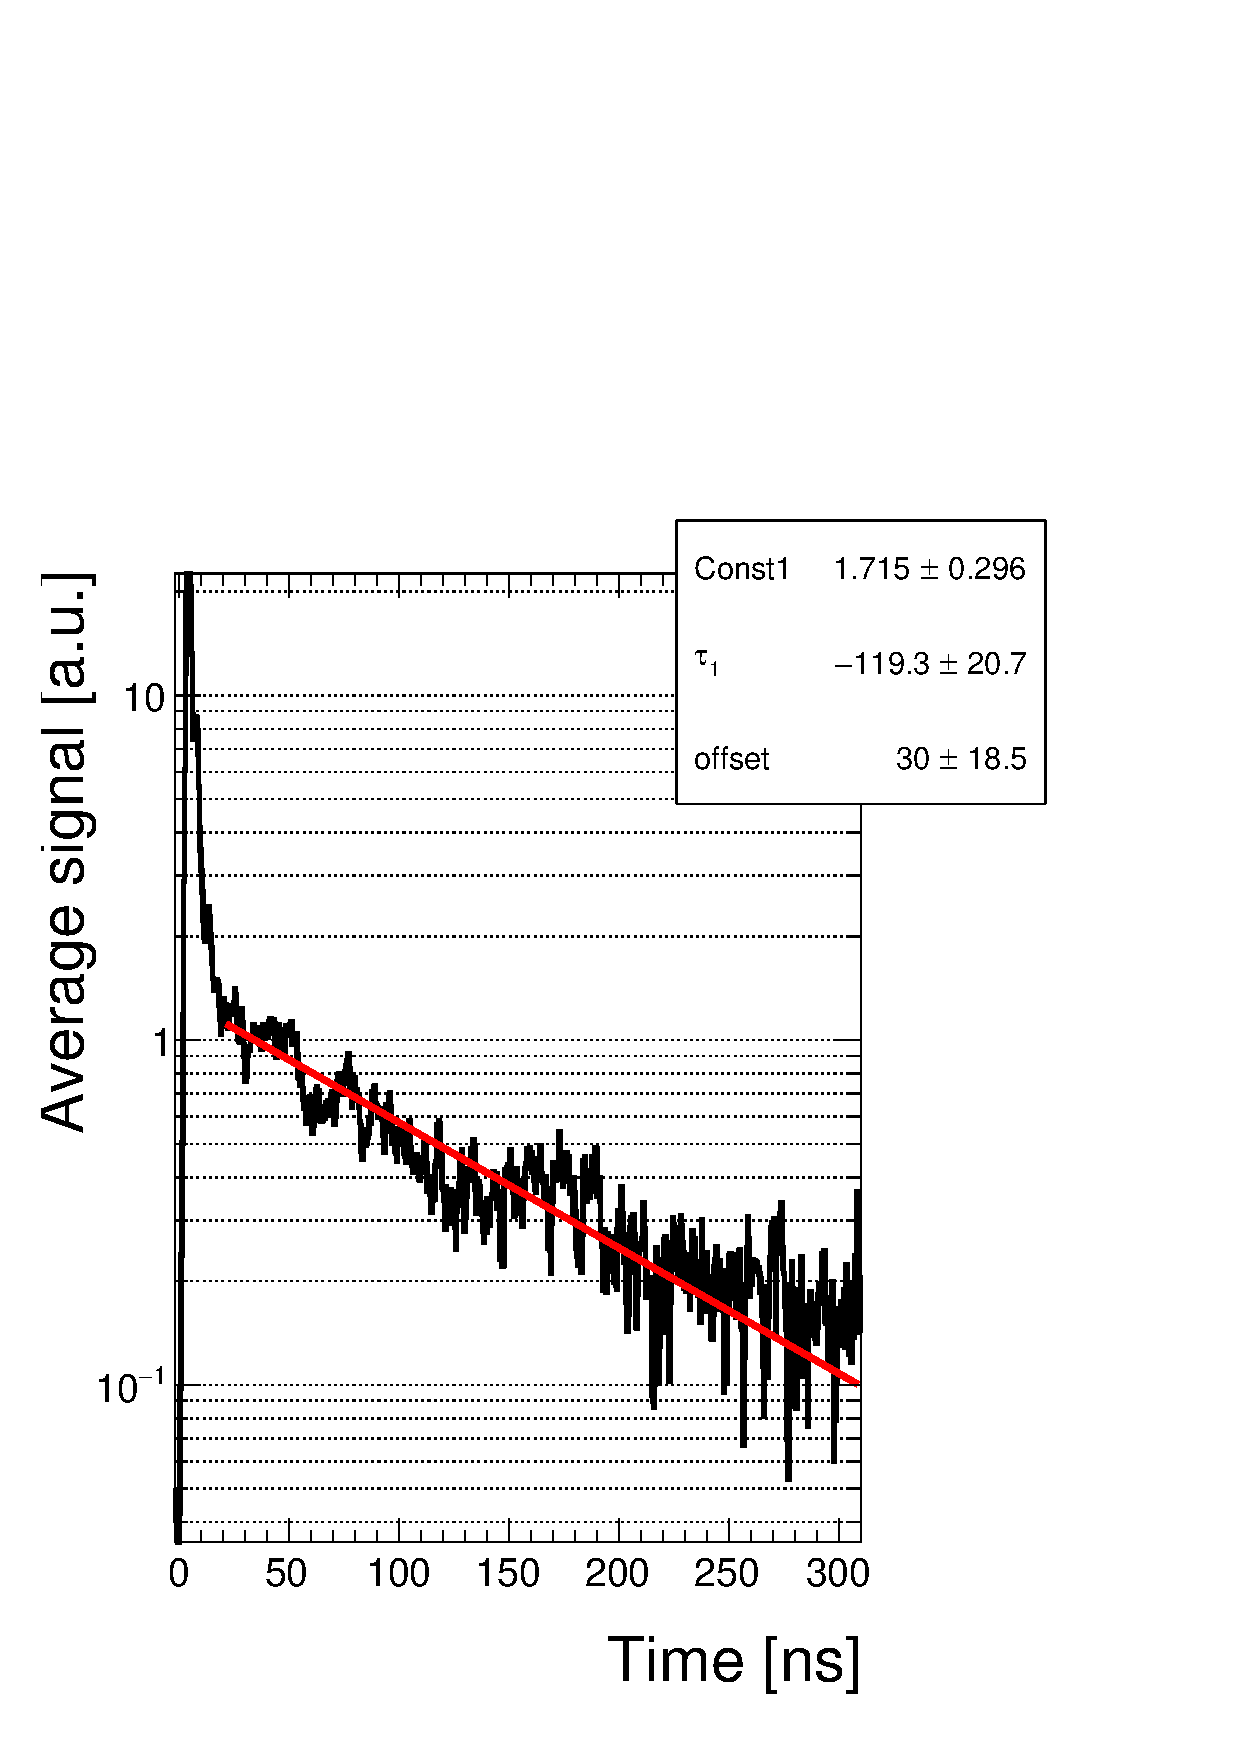
\includegraphics[width=7cm]{Figures/B5_R11864_fit_zoom_singleLog.pdf}
      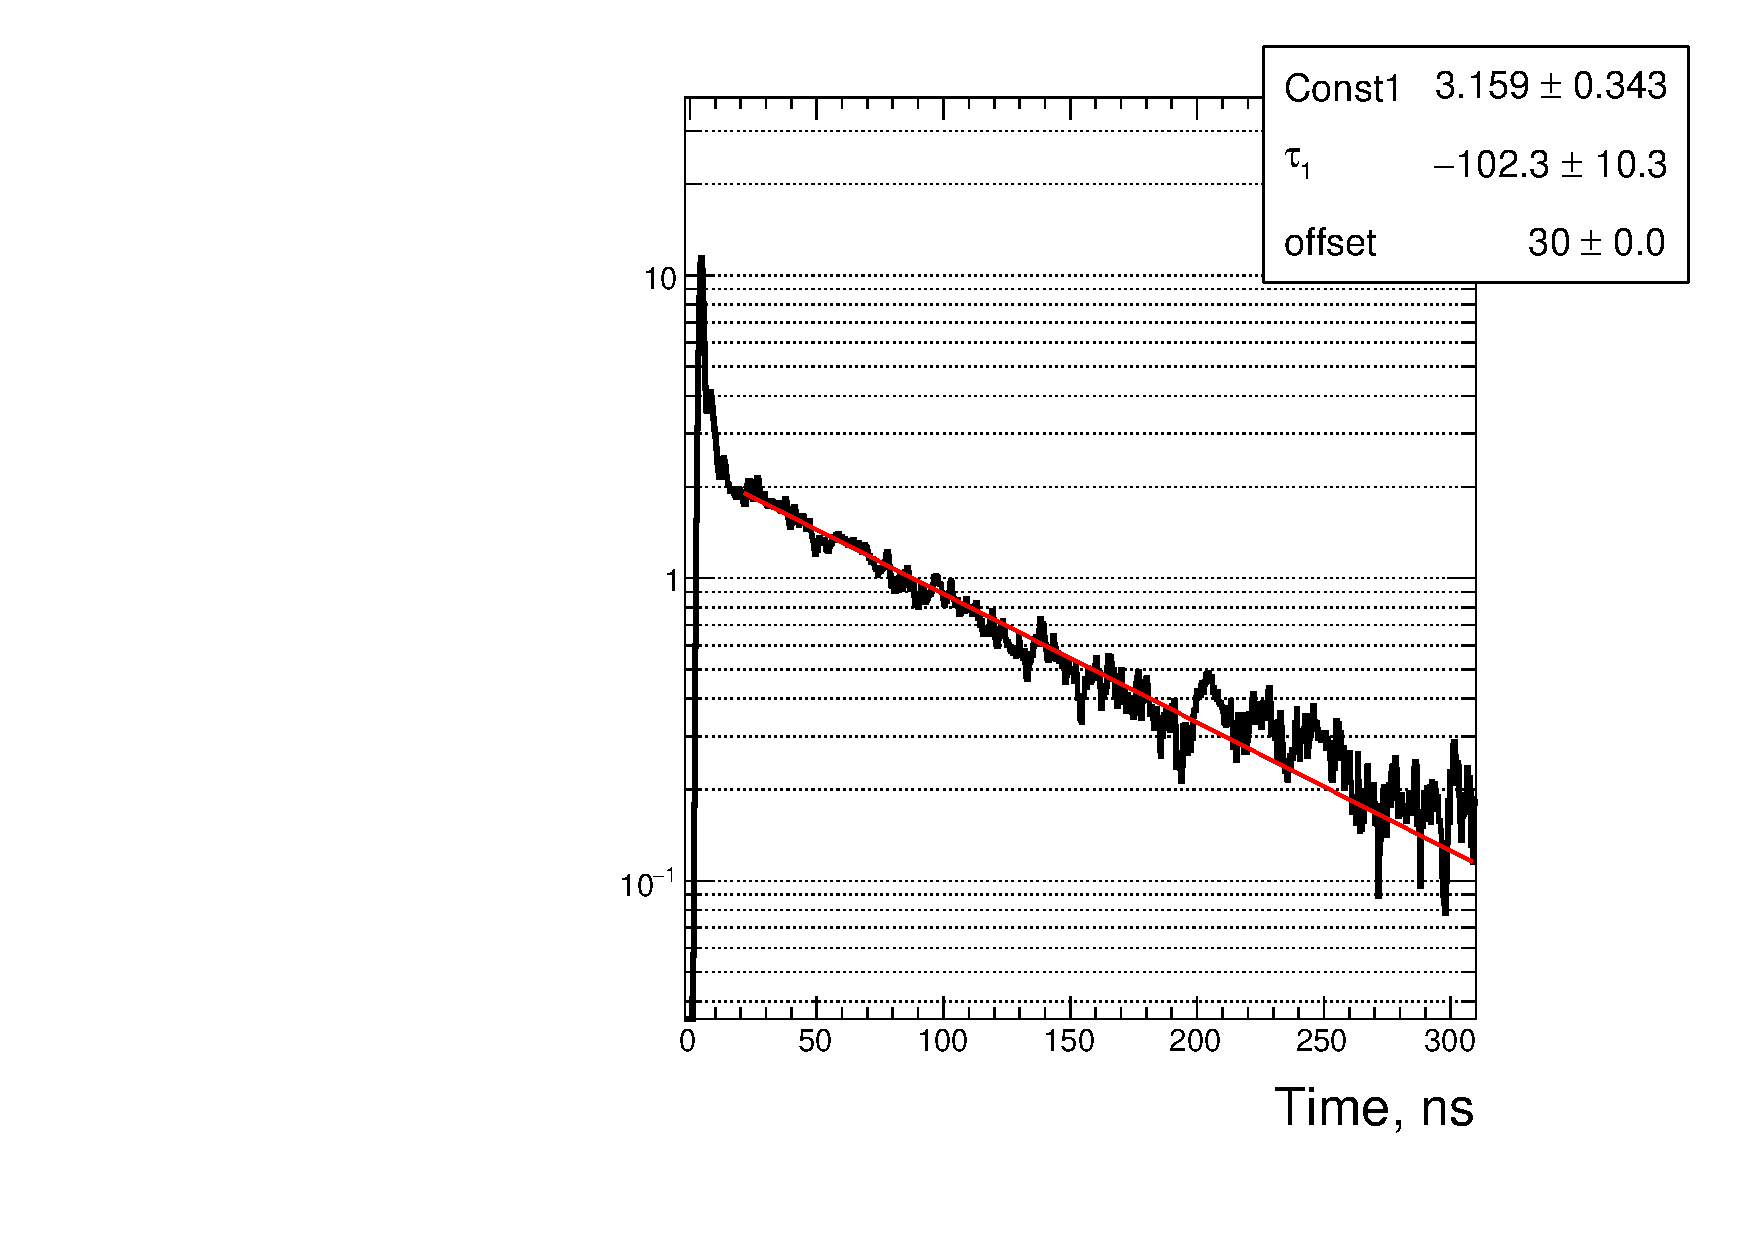
\includegraphics[width=7cm]{Figures/B4_R11863_fit_zoom_singleLog.pdf}
       %%\vspace{-1pc}
\caption{\small The average signal from Phase-IV unirradiated (left) and irradiated (right) fibers. The tail of the scintillation signal is well described by a single exponential (red line) with a time constant of $119.3 \pm 20.7$ ns and $102.3 \pm 10.3$ ns respectively.}
    \label{fig:phase4scintTime}
\end{center}
\end{figure}

%R11864, phase4 unirradiated in front
%SPE 525.213 +/- 10.6236
%Q [p.e] = 0.0924285
%S [p.e] = 0.14725
%S/Q = 1.59313

%R11863, phase4 irradiate in front
%SPE 389.125 +/- 7.04617
%Q [p.e] = 0.0578348
%S [p.e] = 0.616969
%S/Q = 10.6678

%Geant4 prediction OD-ID=15um: 
%Cherenkov : 0.131 p.e./evt
%Scintillation: 0.061 p.e./evt
%S/Q = 0.47
%NB: G4 simulation has OD-ID = 15um for the ce-doped ring . In reality the OR-IR = 15um. Thus the S in this G4 setup is twice smaller and S/Q is twice lower than it should be - to be corrected if this G4 prediction is used. ( JD - 18 Oct 2018)

\section{Ce-doped Fibers Coupled to a CeF\texorpdfstring{$_3$}{} Crystal}
\label{sec:WLS}
Cerium fluoride is an intrinsic scintillator with density $\rho=6.16\; {\mathrm{g/cm}}^3$, radiation length $X_{\rm o} = 1.68$ cm, Moli\`ere radius $R_{\rm M} = 2.6$ cm, nuclear interaction length $\lambda_{\rm I} = 25.9$ cm and refractive index $n = 1.68$, whose luminescence has been discovered by F.A. Kr\"oger and J.~Bakker~\cite{r-KRO} in 1941. In the 1990's, it was extensively studied by D.~F.~Anderson~\cite{r-AND}, W.~W.~Moses and S.~E.~Derenzo~\cite{r-MOS} as a bright and relatively fast scintillator, with decay time constants of 10 - 30~ns. 
%It was adopted as baseline material for the CMS~\cite{r-LOI} and L3P~\cite{r-L3P} electromagnetic calorimeters in their Letters of Intent 
%and thus was extensively studied in high-energy beams~\cite{r-CEFTB}.  For electromagnetic calorimetry in the CMS detector \cite{Nessi2014} after the High-Luminosity upgrade of the Large Hadron Collider at CERN (HL-LHC),
Cerium fluoride was considered for electromagnetic calorimetry in CMS for the HL-LHC, because it recovers from radiation damage~\cite{r-NIMCEF3}, while other crystals, like lead tungstate and LYSO, experience a cumulative damage due to hadrons~\cite{r-FISSNIM, r-NIMLYSO}. A sampling calorimeter design was proposed, alternating tungsten as absorber and cerium fluoride as scintillating medium, with a readout through wavelength-shifting cerium-doped quartz fibers along the chamfers of each calorimeter cell~\cite{r-CALORCEF3, r-WCEF3FRA, r-WCEF3H4}. The choice was made possible by the fact that cerium fluoride broadly emits between 300 nm and 400 nm (Fig.~\ref{fig:cef3spectrum}), with spectrum shape variations depending on the presence of dopants~\cite{r-EACEF3}, conveniently right in the domain of wavelengths that excite the photoluminescent emission of cerium-doped fused-silica~\cite{r-TTU,r-vedda}.

For the test presented herein, a small block of cerium fluoride crystal was used, of dimensions $33\times 24 \times13$ mm$^3$. All its surfaces were unpolished and diffusive to maximize the amount of scintillation light escaping the scintillator and entering the fibers. White, diffusive Tyvek was wrapped around the four larger faces of the crystal, to minimize the amount of scintillation light lost through them. The face opposite the one exposed to the fibers was left unwrapped, to minimize the amount of scintillation light reflected back into the crystal, which has the longest path to the fibers thus the potentially the worst effect on the fast scintillation pulse shape.

\begin{figure}[ht]
\begin{center}
      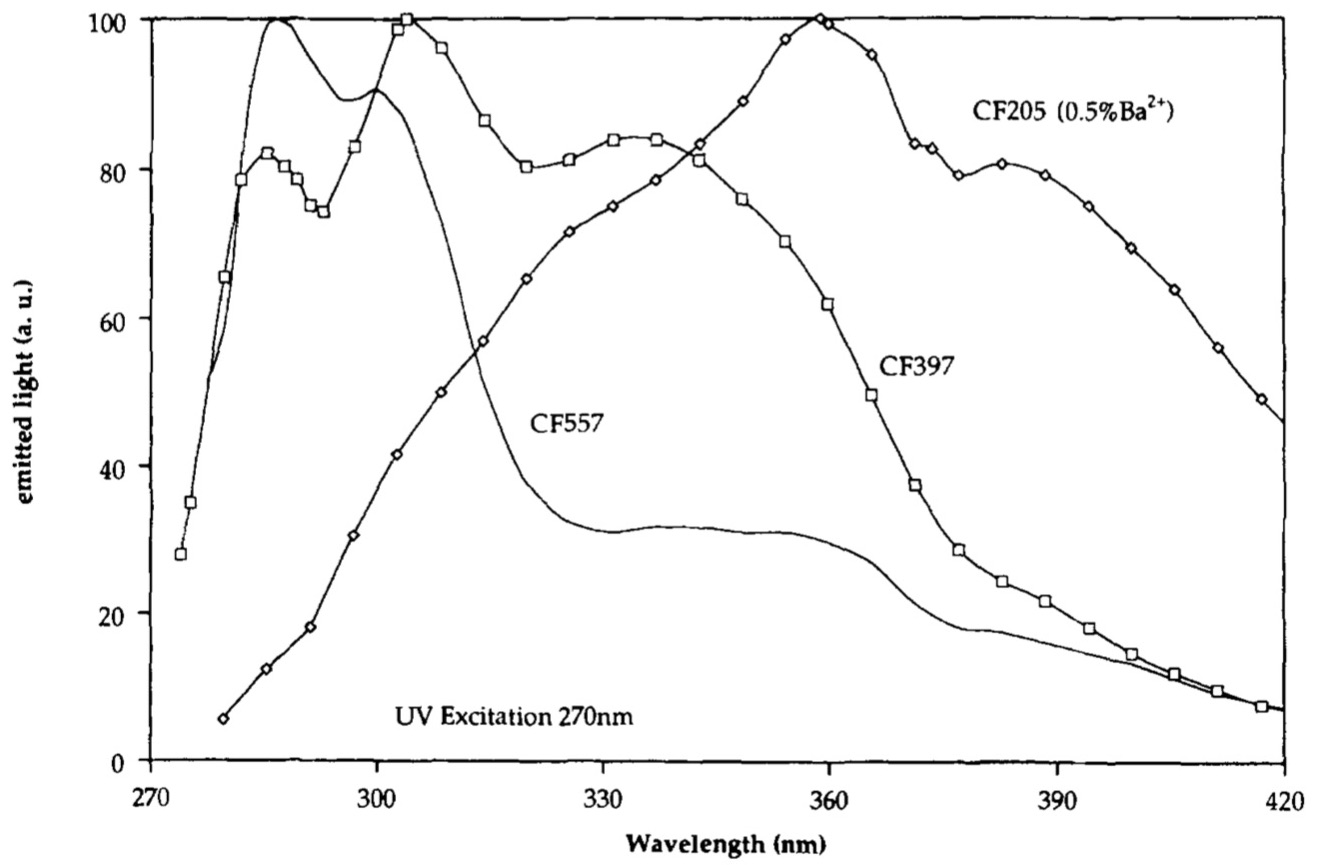
\includegraphics[width=10cm]{Figures/SpectrumCeF3.jpg}
       %%\vspace{-1pc}
\caption{\small Photoluminescence spectra for different CeF$_3$ crystals.}
    \label{fig:cef3spectrum}
\end{center}
\end{figure}


\begin{figure}[ht]
\begin{center}\vspace{-1pc}
      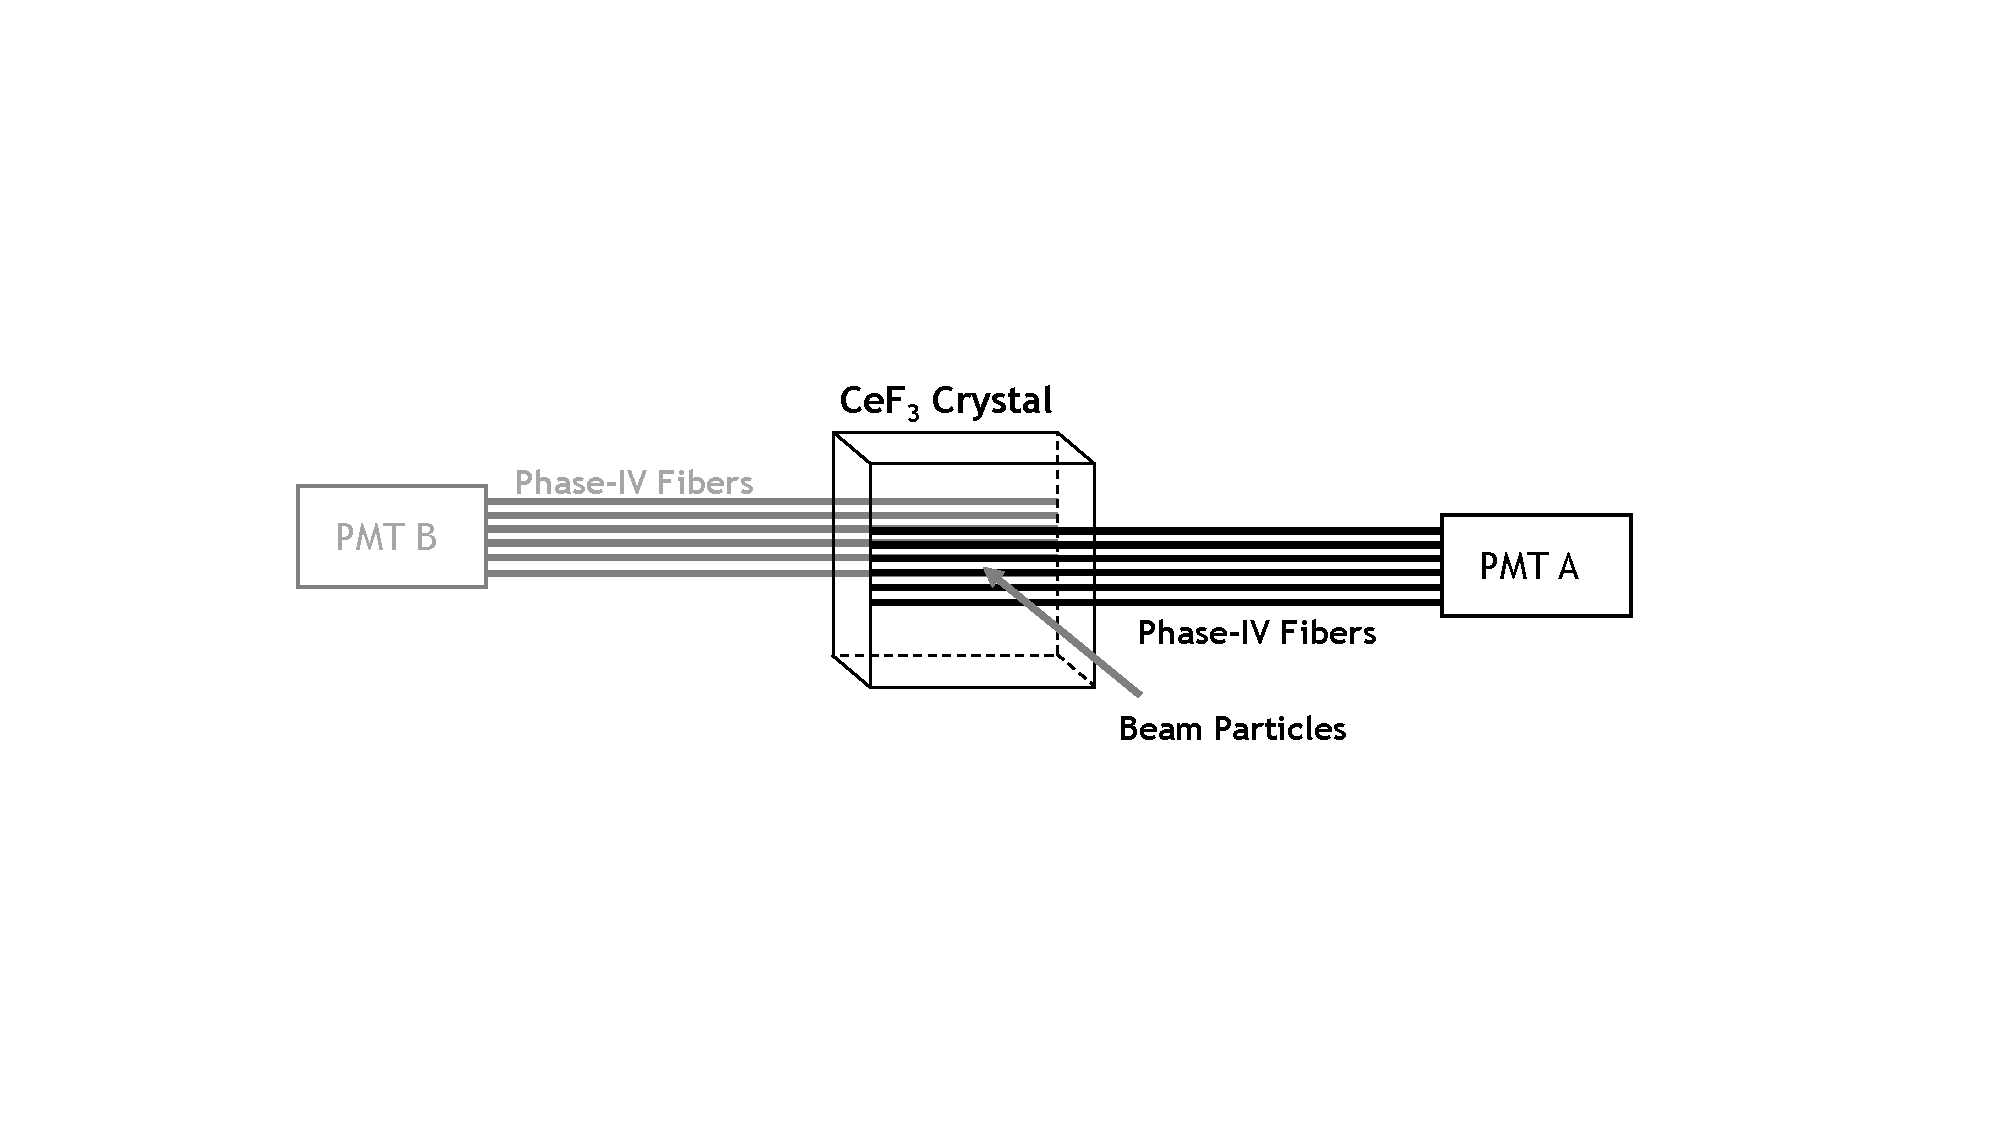
\includegraphics[width=10 cm]{Figures/CeF3Arrangement.pdf}
\caption{\small Arrangement of the fibres with respect to the CeF$_3$ crystal.}
    \label{fig:CeF3Arrangement}
\end{center}
\end{figure}

Two sets of six fibers were air-coupled to the larger one of the crystal surfaces without optical grease and held in place by a tightly wrapped Tyvek sheet as shown in Figure~\ref{fig:CeF3Arrangement}.   One set of six consisted of un-irradiated and the other one consisted of irradiated Phase-IV fibers that were viewed independently by photomultiplier tubes (Hamamatsu R6427).  Irradiated fibers had been exposed to 10 MRad of gamma irradiation three months prior to these measurements and some optical recovery had occurred.  For cross calibration purposes between the two channels, the PMTs and the orientation of fibers on the crystal surfaces with respect to the beam direction were swapped in all possible (4) combinations.  

Figure~\ref{fig:CeF3signals} shows the measured spectra where the fast part (0-50 ns) of the spectra is clearly different and the irradiated fibers have lost sensitivity to this temporal region of light emission from the crystal.  In the longer time scales (>50 ns), the tail of the signal is essentially the same (XX ns).

\begin{figure}[ht]
\begin{center}
      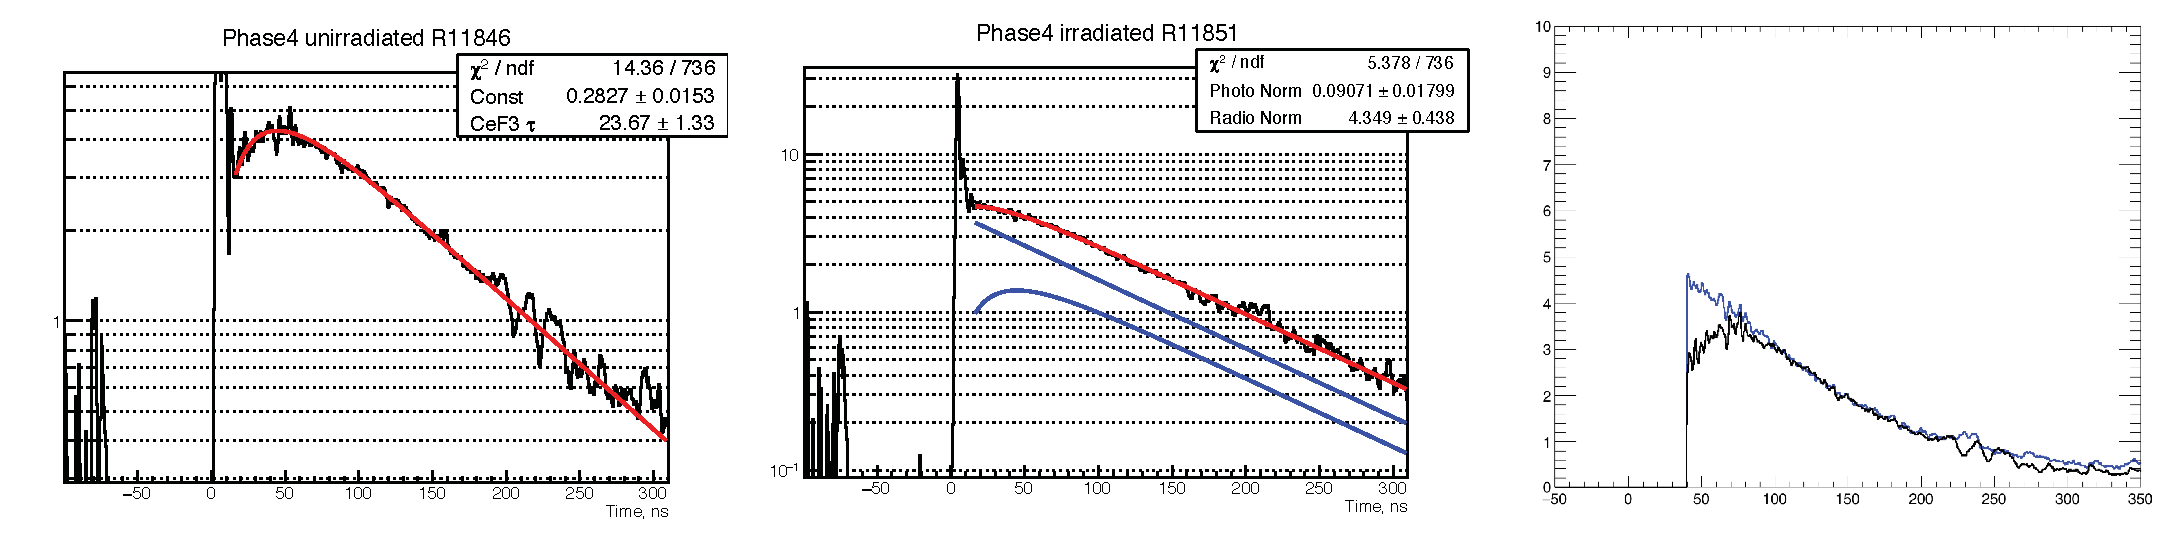
\includegraphics[width=14cm]{Figures/CeF3coupledFibers.pdf}
       %%\vspace{-1pc}
\caption{\small The averaged signals from the CeF$_3$ crystal coupled to either un-irradiated (left) or irradiated (middle) fibers display a significant difference at the short time scale (0-50 ns).  The right plot shows the overlaid spectra when the two channels are calibrated for the same PMT gain.  The red curve ...  the blue curve...}
    \label{fig:CeF3signals}
\end{center}
\end{figure}


\subsection{Scintillation light analysis (temporary placeholder for text edits)}

  CeF$_3$ crystal with Phase-IV fibers attached to it were exposed to electron beam with energy of 16 GeV. The PMT signals were read-out by a fast digitizer (CAEN V1742) at 2.5 GHz and a common trigger was generated by a fast multichannel photomultiplier (MCP). Figure~\ref{fig:CeF3signals} shows the measured spectra where the fast part (0-50 ns) of the spectra is clearly different and the irradiated fibers have lost sensitivity to this temporal region of light emission from the crystal.  In the longer time scales (>50 ns), the tail of the signal is essentially the same (XX ns). The scintillation light in this configuration has two components - photo-luminescence and radio-luminescence. The radio-luminescence results from particle passing trough the Ce-doped ring of the fibers. The timing characteristics of the two components of the scintillation signal differ due to the presence of comparable scintillation decay time in the CeF$_3$ crystal ($\sim 24$ ns) in the photo-luminescence component. We use analytic functions to model the photo-luminescence and radio-luminescence contributions to the observed signal. We fit this model to the data to extract the relative contributions in the measured signal. The data from the un-irradiated Phase-IV fiber is best described by model with $\sim 100$\% contribution from the photo-luminescence, while the data for irradiated Phase-IV fiber suggest that only a 1/4 of the total signal is from  photo-luminescence. Furthermore we cross-reference this model prediction with the S/Q measurement without CeF$_3$ crystal and we found it to be in reasonable agreement, confirming sizable radio-luminescence contribution. 

\section{Timing Measurements}
\label{sec:timing}
In addition to the light yield studies presented in the previous section, an attempt to characterize the timing performance of the cerium-doped fibers was carried out. The fibers show a direct and fast Cherenkov component, well separated from the scintillation one. In the context of calorimetry at the hadron colliders, studies indicate that precise timing information (tens of ps) is beneficial for pile-up mitigation and for the correct assignment of physics objects to their primary vertices. It becomes then interesting to exploit the Cherenkov signal for timing applications.  The relative abundance of the light generated via Cherenkov processes and then collected, strongly depends on the orientation of the fibers with respect to the direction of development of the showers. In the setup considered, the fibers are positioned at 90 degrees with respect to the beam direction and only the Cherenkov photons emitted within the numerical aperture of the fiber are guided to the photosensor via total internal reflection.

In order to measure the time resolution of the fibers, two MCP photosensors were placed directly on the beam axis and used as a time reference. For each pulse shape the timing is defined as the position of the time sample corresponding to half of the pulse's maximum amplitude mimicking a constant fraction discriminator (CFD) at 50\%. The timing performance was then measured by fitting the distribution of $(t_{\rm MCP} - t_{\rm fiber})$ in bins of charge with a gaussian function.  The time resolution can be expressed as the sum in quadrature of two terms accounting for different sources of uncertainty and can be parametrized as follows:
\begin{equation}
    \sigma^2(t) = \bigg( \frac{S}{\sqrt{A}} \bigg)^2 + C^2
\end{equation}
where $A$ is the measured amplitude while $S$ and $C$ are the stochastic and constant term coefficients, respectively. For MCPs, the measured constant term was 17~ps, consistent with the expected performance form the MCP specs.

Following the same approach, the time resolution for the fibers (Phase-IV irradiated, Phase-IV un-irradiated and clear fused-silica fiber) was measured and compared to the performance of a plastic scintillating fiber that doesn't exhibit a Cherenkov peak (Figure~\ref{fig:fibres_time_res}).

\begin{figure}[ht]
\begin{center}\vspace{-1pc}
      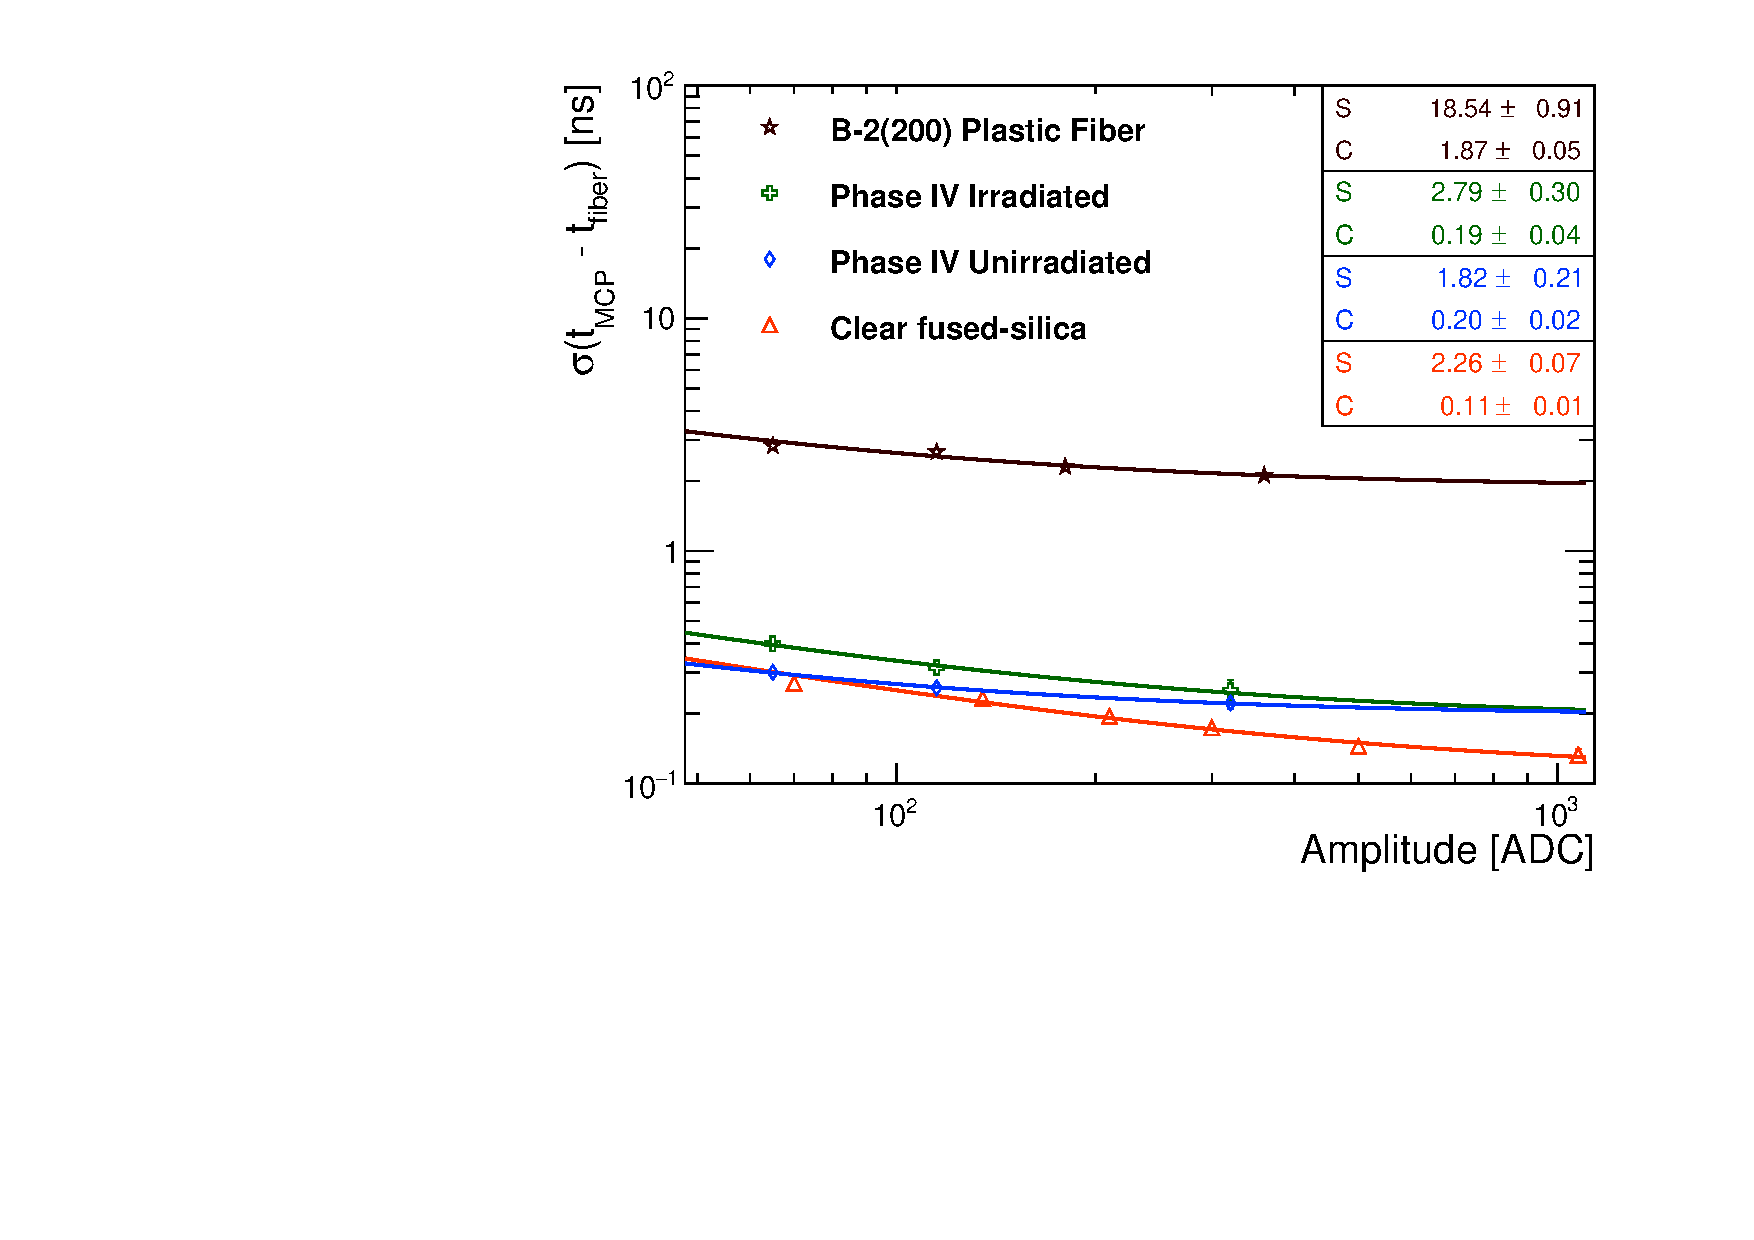
\includegraphics[width=12cm]{Figures/fibres_time_res}
       %%\vspace{-1pc}
\caption{\small Time resolution curves for different types of fibers. The MCP photodetectors are used as time reference.  One ADC count equals XXX pC.}
    \label{fig:fibres_time_res}
\end{center}
\end{figure}
The following observations were made:
\begin{itemize}
\item there is a clear advantage in using Cherenkov light for timing measurements compared to slower scintillation light. For the setup considered, where very few photoelectrons are generated per event, promptly produced photons guarantee a time resolution which is not degraded by the slower light re-emission from scintillation processes;
\item in the hypothesis of an infinite number of photoelectrons, the cerium-doped fused-silica fibers and the scintillation plastic fibers are expected to have the same timing performance if they are read out with the same photodetector. The measurements performed, however, do not allow a proper measurement of the constant term in some cases due to the low signal;
\item irradiated vs un-irradiated Phase-IV fiber?  Does it scale like e$^-2$?  Is it just photostatistics?
\item what is to be said about the plastic scintillating fiber?
\item having a transit time spread of 500~ps (FWHM), the PMTs used in these studies are not well suited for timing measurements. The timing resolution measurement for the fibers in this case is limited by the PMT resolution.
\end{itemize}
In conclusion, it becomes clear that to be able to project the observed time performance to a realistic case for applications in future calorimeters, a different setup and a different readout would be needed. Nevertheless, the observation of a clean Cherenkov component in the pulses are interesting and are to be investigated for high-precision timing measurements.

\section{Conclusions}
\label{sec:conclusions}

%%
%%  Conclusion from the first JINST paper below:
%%
%The need for radiation-hard scintillators beyond what it available today is the primary reason to explore the type of
%hybrid fiber described here.  The clear fused-silica fibers, because of their
%superior radiation-hardness, are good candidates to host luminescent dyes.  The choice of cerium~\cite{Blasse}, one of the most commonly employed dyes in the scintillator industry,
%as a starting point was based on its apparent high light yield, its peak emission wavelength appropriate for standard PMTs, and its potential radiation hardness.   As much as twice the light yield compared to the Bi$_3$Ge$_4$O$_{12}$ (BGO) \cite{Chiodini2002} and tolerance
%to $\sim$100 kGy  was reported  in some cerium-doped ingots \cite{Vedda2006}.  Other rare earth
%materials can also be used as dyes.  Praseodymium, for example, is faster ($\sim$ 20 ns), with an emission peak at a shorter wavelength (308 nm) compared to cerium \cite{Pejchal2009,Sun2012}.  Both the emission spectrum and the decay times may be modified by the introduction of co-dopants, an area we wish to explore.
%
%Silica fibers doped in this way offer an interesting feature: they do not contain much hydrogen.  This property may have a useful implication, especially for calorimetry.  Event-by-event compensation results in a significant performance improvement when plastic scintillating and clear fibers are used in dual-readout calorimetry.  Because the clear (Cherenkov) fibers are mainly sensitive to the electromagnetic core of hadronic showers, it is possible to keep track of the large fluctuation in $\pi^0$ production in hadronic showers event by event, and effectively to compensate ($e/h=1$) the energy measurement. If, in addition to plastic scintillating fibers, rare earth doped fibers such as Phase-II fibers are introduced in a triple-readout scheme, then it is possible to track the next largest fluctuation, {\it i.e.} the fluctuations originating from binding energy losses in nuclear break-up, by measuring the neutrons of a few MeV.   In principle, this can be accomplished by measuring the signal difference between the two scintillating (hydrogenous {\it vs} non-hydrogenous) fibers on an event-by-event basis.
%
%As we already demonstrated, cerium-doped fibers are well-suited as WLS fibers for CeF$_3$
%\cite{Nessi2014}.  There is a substantial overlap between the excitation  of the SiO$_2$:Ce$^{3+}$ and the emission bands of the CeF$_3$.

%If we succeed in improving the radiation hardness of these fibers beyond plastics, we will have already achieved a significant improvement.

%Relevant fundamental and practical questions appear to involve level of radiation-hardness and cost.  As to the first, we have made some tangible progress.  As to the second, the initial cost estimate of cerium-doped fused-silica fibers by Polymicro is less than 1\$/m for 600 $\mu$m core fibers in large (over 10,000 km) quantities, similar to clear fused-silica fibers.

\section{Acknowledgements}
This work has been supported by the US Department of Energy, Office of Science (DE-SC001592), the Akdeniz University Scientific Research Projects Coordination Department (FDK-2017-2461), and the Scientific and Technological Research Council of Turkey, T\"UBITAK, (No. 1059B141601412). The project has also been supported by European Union's Horizon 2020 research and innovation program under the grant agreement N$^\circ$654168 (AIDA 2020). We express our thanks to Etiennette Auffray-Hillemanns for generously sharing the beam time at CERN. Jim Clarkin and Teo Tichindelean from Polymicro Technologies are thanked for their expertise, continued interest, and commitment to this R\&D project.


% We suggest to always provide author, title and journal data:
% in short all the informations that clearly identify a document.
\bibliographystyle{JHEP}
\bibliography{mybibfile}
\end{document}